\section{Identifying Common Measures of Feature Importance for Nonlinear Ground Truth Models}
\label{sec:general_case}
\textcolor{red}{In the preceding sections, we constructed an intended estimand—the true marginal effects ($\boldsymbol{\beta}$)—using a linear simulated dataset and compared it against post hoc explainers (LIME/SHAP) through three metrics: directionality, concordance, and relevance. However, this linear scenario alone may insufficiently capture the potential misalignment between explainers and underlying -generating mechanisms. To address this limitation, we present an extended analysis in this section.}

\textcolor{red}{Specifically, Section \ref{sec:nonlinear data generation} introduces multiple nonlinear simulated datasets, emphasizing key vary factors in their generation. Section \ref{sec:intended estimands} extends the evaluation framework by proposing four additional Intended estimands in these nonlinear settings. Section \ref{sec:metrics} formalizes new metrics to quantify discrepancies between post hoc explanations and the proposed estimands. Finally, Section \ref{sec:nonlinear results} evaluates the performance of these metrics across datasets, analyzing their relationships with the vary data-generating factors.}

\subsection{Data Generation}
    \label{sec:nonlinear data generation}
% vary factor of building G, data
% how we trained M
\textcolor{red}{Building upon the linear analysis in previous sections, we now extend our evaluation to nonlinear settings through controlled synthetic data generation. This comprehensive approach allows us to systematically investigate how varying data characteristics influence post hoc explainer performance. The process encompasses three core components: nonlinear dataset generation, ground truth model establishment(model $\mathcal{G}$), and black-box model training(model $\mathcal{M}$), which collectively enable a more complete assessment of explanation methods' capabilities and limitations.}

\textcolor{red}{To initiate this analysis, we first constructed 81 distinct binary classification datasets with configurable nonlinearities. As summarized in Table~\ref{tab:data_factors}, these datasets were generated by exhaustively combining four vary factors while maintaining two fixed facotrs. The sample size was held constant at 5,000 instances to ensure statistical reliability, and Gaussian noise with standard deviation 0.1 was added to simulate real-world measurement variability. Notably, the variable factors were carefully selected to span realistic scenarios: feature dimensionality (10-30 features), correlation strength ($\rho \in \{0, 0.5, 1\}$), and nonlinear complexity (0-10 quadratic terms and interaction terms respectively). This design enables us to later examine how these fundamental data properties affect explanation fidelity.}

\begin{table}[htbp]
\centering
\caption{Data Generation Factors and Configurations}
\label{tab:data_factors}
\begin{tabular}{lllc}
\toprule
\textbf{Factor} & \textbf{Variable} & \textbf{Type} & \textbf{Values} \\
\midrule
Sample size & \texttt{Num\_instance} & Fixed & 5,000 \\
Noise std. dev. & \texttt{Noise\_std} & Fixed & 0.1 \\
Number of features & \texttt{Num\_feature} & Varied & 10, 20, 30 \\
Correlation strength & \texttt{Corr\_strength} & Varied & 0, 0.5, 1 \\
Nonlinear terms & \texttt{Nonlinear\_num} & Varied & 0, 5, 10 \\
Interaction terms & \texttt{Interaction\_num} & Varied & 0, 5, 10 \\
\bottomrule
\end{tabular}
\end{table}

\textcolor{red}{Transitioning from parameter specification to implementation, each dataset $\mathcal{D}_i$ was generated through a rigorous seven-step process (detailed in Algorithm~\ref{app:nonlinear_data_generation} in appendix) that mirrors realistic data structures. Beginning with $m-1$ independent $\mathcal{N}(0,1)$ features, we introduced controlled correlations through an $m$-th feature generated via $\rho$-dependent linear combinations. The nonlinear components were then systematically incorporated through quadratic transformations of $p$ selected features and pairwise interactions between $q$ feature combinations. To establish known ground truth for interpretability validation, we assigned uniformly distributed coefficients ($C \sim \text{Uniform}(-1,1)$) to all terms before computing response probabilities through a noisy sigmoid transformation. The final balanced datasets, comprising $m + p + q$ features each, were thresholded to yield binary classifications while maintaining equal class representation.}

\textcolor{red}{Having established the data generation framework, we now turn our attention to model construction (detailed in Algorithm~\ref{app:constuction models} in Appendix). The first model class, designated Model $\mathcal{G}$, serves as our ground truth benchmark by precisely replicating each dataset's generation mechanism. Implemented as scikit-learn Pipelines, these 81 models ($\mathcal{G}_1$ through $\mathcal{G}_{81}$) incorporate identical nonlinear transformations and fixed coefficients as their corresponding datasets. This exact correspondence guarantees that Model $\mathcal{G}$'s explanations reflect the true data-generating process, providing an essential reference point for subsequent explainer evaluations.}

\begin{table}[htbp]
\centering
\caption{Model Specifications}
\label{tab:models}
\begin{tabular}{lll}
\toprule
\textbf{Model} & \textbf{Purpose} & \textbf{Specification} \\
\midrule
Model $\mathcal{G}$ & Ground truth & Logistic regression with exact data-generating parameters \\
Model $\mathcal{M}$ & Black box & XGBoost with performance-stratified variants \\
\bottomrule
\end{tabular}
\end{table}

\textcolor{red}{To complement these idealized models and simulate practical machine learning scenarios, we developed Model M as a collection of performance-stratified XGBoost implementations. For each of the 81 datasets, we trained 12 distinct variants (totaling 972 models) by systematically varying both training set size (50-80\% of data) and key hyperparameters(max\_depth and n\_estimators). As detailed in Table~\ref{tab:models}, these models were intentionally distributed across four accuracy brackets ([0.7,0.75), [0.75,0.8), [0.8,0.85), and [0.85,0.9]) to enable robust analysis of performance-dependent explanation quality. This two-tiered modeling approach - combining perfectly specified Model $\mathcal{G}$ with realistically trained Model $\mathcal{M}$ - creates a comprehensive testbed for evaluating post hoc explainers under both idealized and practical conditions.}

\textcolor{red}{In summary, our experimental design ultimately considers five varying factors: \texttt{Number of features}, \texttt{Correlation strength}, \texttt{Nonlinear terms}, \texttt{Interaction terms}, and \texttt{Accuracy}. The first four correspond to the variable parameters in the synthetic data generation process, while the last factor (\texttt{Accuracy}) arises from the controlled variation of Model~$\mathcal{M}$'s performance through training data size and hyperparameter adjustments. In the following subsections, we systematically examine how changes in these factors influence the divergence between post hoc explainer outputs and the ground-truth explanations derived from Model~$\mathcal{G}$.}

\subsection{Intended Estimands}
\label{sec:intended estimands}
% \paragraph{Intended Estimand} - "what do researcher use Shapley value for? how do they use it?"
% Reviewers complain that we conflate marginal effect with shapley value, and argue that researchers could have meant sth else, such as predictive power, not really marginal value. That's why we included more estimands, such that we can claim "no matter what authors meant, it is incorrect to infer anything on data from M"
% \begin{itemize}
%     \item Marginal Effect
%     \item Shapley value of G
%     \item Drop in accuracy of M
%     \item Success Rate
% \end{itemize}

\textcolor{red}{To establish a comprehensive framework for evaluating post hoc explanation methods, we define three intended estimands. This multi-faceted approach is motivated by the fundamental ambiguity in what explanation methods like SHAP actually measure in practice - whether they reflect true marginal effects, predictive contributions, or other notions of feature influence. By formally characterizing ground truth explanations ($\tau_1$), predictive power through ablation ($\tau_2$), and counterfactual validity ($\tau_3$), we create the necessary foundation to systematically examine how different interpretation methods perform across these conceptually distinct dimensions of interpretability.}

\subsubsection*{Ground truth explanations}
\textcolor{red}{The primary estimand $\tau_1$ represents the \textit{ground truth explanations} derived from Model $\mathcal{G}$ ($\mathcal{G}_x$), whose parameters are specified to match the data-generating process of $\mathcal{D}_x$. This estimand is obtained by applying post hoc explainers (LIME/SHAP) to $\mathcal{G}_x$ on its corresponding dataset $\mathcal{D}_x$. For any test sample $i$ in $\mathcal{D}_x$, the explanation vector is formally defined as:}

\begin{equation}
    \tau_1 = e_{i}^{\mathcal{G}_x,\text{LIME/SHAP}} = (v_{1}^{\mathcal{G}_x,\text{LIME/SHAP}}, \ldots, v_{m}^{\mathcal{G}_x,\text{LIME/SHAP}})
\end{equation}

\textcolor{red}{where $m$ is the number of features and $v_k$ denotes the explanation value for the $k$-th feature. The absolute value of each dimension in the vector indicates the relative importance of the corresponding feature, with larger absolute values signifying greater importance as assessed by the explainer based on Model $\mathcal{G}$ and dataset $\mathcal{D}_x$. These explanations serve as our reference standard, as Model $\mathcal{G}$'s parameters correspond to the known data-generating parameters.}

\subsubsection*{Predictive Power through Ablation}
\textcolor{red}{The second estimand $\tau_2$ quantifies the \textit{predictive importance} of features through accuracy reduction when features are removed from Model $\mathcal{M}$ ($\mathcal{M}_x^j$). For each feature k, we compute:}

\begin{equation}
    \tau_2 = d_k^{\mathcal{M}_x^j} = \text{Accuracy}(\mathcal{M}_x^j) - \text{Accuracy}(\mathcal{M}_x^j \setminus \text{feature } k)
\end{equation}

\textcolor{red}{yielding an accuracy decrement vector:}
\begin{equation}
    \mathbf{d}^{\mathcal{M}_x^j} = (d_1^{\mathcal{M}_x^j}, \ldots, d_m^{\mathcal{M}_x^j})
\label{equation:accuracy decrements}
\end{equation}

\textcolor{red}{This estimand captures how essential each feature is for the model's predictive performance, independent of explanation methods.}

\subsubsection*{Counterfactual validity}
\textcolor{red}{The third estimand $\tau_3$ evaluates whether top-$k$ important features identified by explanations can generate valid counterfactuals in Model $\mathcal{G}$. Specifically, we use post hoc explainers (LIME/SHAP) with Model $\mathcal{M}$ to define the top-k most important features, then assess with Model $\mathcal{G}$ and the DICE algorithm whether valid counterfactuals can be generated when only these features are allowed to vary. For a test sample $x^{(s)}$ and top-k features $\text{Top}_k = \{i_1,\ldots,i_k\}$, we define:}

\begin{equation}
    \tau_3 = \mathbb{I}\left(\exists x_{\text{cf}}^{(s)} \text{ s.t. } \mathcal{G}_x(x_{\text{cf}}^{(s)}) \neq \mathcal{G}_x(x^{(s)}) \land x_{\text{cf},j}^{(s)} = x_j^{(s)}\ \forall j \notin \text{Top}_k\right)
\end{equation}

\subsection{Evaluation Metrics}
% \paragraph{Metrics} Metrics refer to \emph{how} we compare shapley value agains each of the intended estimand. In the previous submission, we used directionality, concordance, and top-k recall. Here we expanded to 
% \begin{itemize}
%     \item rank correlatino
%     \item kendal 
%     \item 
% \end{itemize}
% \subsection{Results}
\label{sec:metrics}

\textcolor{red}{We develop four metrics to evaluate how post hoc explanations from Model $\mathcal{M}$ align with our intended estimands ($\tau_1$, $\tau_2$, $\tau_3$). As summarized in Table~\ref{tab:metric_relationship}, each metric assesses a different dimension of explanation quality by comparing specific estimand pairs.}

\subsubsection*{Global Ranking Correlation}
\textcolor{red}{This metric evaluates dataset-level agreement between Model M's explanations and the ground truth estimand $\tau_1$. We compute two variants:}

\textcolor{red}{The Spearman rank correlation version:}
\begin{equation}
\text{GlobalCorr}_{\text{Spearman}} = 1 - \frac{6\sum_{j=1}^D (r^{\mathcal{G}_x}_j - r^{\mathcal{M}_x^j}_j)^2}{D(D^2-1)}
\end{equation}
\textcolor{red}{where $D$ is the number of features, $r^{\mathcal{G}_x}_j = \text{Rank}_j(\frac{1}{S}\sum_{i=1}^S |e_i^{\mathcal{G}_x,\text{LIME/SHAP}}|)$ is the ground truth rank of the $j^{\text{th}}$ feature, and $r^{\mathcal{M}_x^j}_j$ is the model's rank assignment. The coefficient ranges in $[-1,1]$, with 1 indicating perfect rank agreement.}

\textcolor{red}{The Kendall's tau version:}
\begin{equation}
\text{GlobalCorr}_{\text{Tau}} = \frac{n_c - n_d}{\sqrt{(n_0 - n_1)(n_0 - n_2)}}
\end{equation}
\textcolor{red}{where $n_c$ and $n_d$ count concordant and discordant feature pairs respectively, $n_0 = D(D-1)/2$ is the maximum possible pairs, with $n_1$, $n_2$ adjusting for tied ranks in $\mathbf{r}^{\mathcal{G}_x}$ and $\mathbf{r}^{\mathcal{M}_x^j}$ respectively.}

\subsubsection*{Local Ranking Correlation}
\textcolor{red}{This measures sample-wise explanation consistency with $\tau_1$, with two variants:}

\textcolor{red}{Spearman correlation across samples:}
\begin{equation}
\text{LocalCorr}_{\text{Spearman}} = \frac{1}{T}\sum_{t=1}^T \left(1 - \frac{6\sum_{k=1}^D (R_{t,k}^{\mathcal{G}_x} - R_{t,k}^{\mathcal{M}_x^j})^2}{D(D^2-1)}\right)
\end{equation}

\textcolor{red}{Kendall's tau across samples:}
\begin{equation}
\text{LocalCorr}_{\text{Tau}} = \frac{1}{T}\sum_{t=1}^T \frac{n_{c,t} - n_{d,t}}{\sqrt{(n_{0,t} - n_{1,t})(n_{0,t} - n_{2,t})}}
\end{equation}

\textcolor{red}{The metrics evaluate feature ranking consistency between ground truth and model explanations for each individual sample. Here $T$ denotes the total number of samples in the evaluation set, while $D$ represents the number of features. For each sample $t$, $R_{t,k}^{\mathcal{G}_x} = \text{Rank}_k(|e_t^{\mathcal{G}_x,\text{LIME/SHAP}}|)$ gives the ground truth ranking of feature importance, where features are ordered by their absolute explanation values. Similarly, $R_{t,k}^{\mathcal{M}_x^j}$ represents Model $\mathcal{M}$'s corresponding feature ranking for the same sample.}

\textcolor{red}{The Spearman correlation computes the average rank correlation across all samples, where perfect agreement ($R_{t,k}^{\mathcal{G}_x} = R_{t,k}^{\mathcal{M}_x^j}$ for all $k$) yields a value of 1. The Kendall's tau variant measures concordance through pairwise comparisons, where $n_{c,t}$ counts the number of feature pairs with consistent relative rankings between ground truth and model explanations for sample $t$, and $n_{d,t}$ counts inconsistent pairs. The denominator terms $n_{1,t}$ and $n_{2,t}$ adjust for tied rankings in the ground truth and model outputs respectively, with $n_{0,t} = D(D-1)/2$ being the total possible feature pairs. Both metrics range from -1 (perfect inversion) to 1 (perfect agreement), with 0 indicating no correlation.}

\subsubsection*{Remove Ranking Correlation}
\textcolor{red}{This evaluates the alignment between $\tau_2$ (predictive importance) and dataset-level feature importance rankings based on Model $\mathcal{M}$'s explanations ($\mathcal{M}_x^j$), computed as:}

\textcolor{red}{Spearman version:}
\begin{equation}
\text{RemoveCorr}_{\text{Spearman}} = 1 - \frac{6\sum_{k=1}^D (r_k^{\text{ablation}} - r_k^{\mathcal{M}_x^{j}})^2}{D(D^2-1)}
\end{equation}

\textcolor{red}{Kendall version:}
\begin{equation}
\text{RemoveCorr}_{\text{Tau}} = \frac{n_c - n_d}{\sqrt{(n_0 - n_1)(n_0 - n_2)}}
\end{equation}

\textcolor{red}{The metrics quantify how well the model's explanation rankings $\mathbf{r}^{\mathcal{M}_x^{j}}$ align with feature importance derived from ablation studies $\mathbf{r}^{\text{ablation}}$, where $D$ is the total number of features. The ablation-based ranks $r_k^{\text{ablation}}$ are obtained by sorting features according to Model $\mathcal{M}$'s accuracy degradation (see Eq.\ref{equation:accuracy decrements}) when each feature is removed, with higher accuracy drops indicating more important features. The explanation ranks $r_k^{\mathcal{M}_x^{j}}$ come from aggregating sample-wise explanation magnitudes across the dataset.}

\textcolor{red}{For the Spearman correlation, perfect alignment ($r_k^{\text{ablation}} = r_k^{\mathcal{M}_x^{j}}$ for all $k$) yields a value of 1, while complete inversion gives -1. The Kendall's tau variant evaluates pairwise rank consistency, where $n_c$ counts feature pairs with matching order in both rankings, and $n_d$ counts discordant pairs. Here $n_0 = D(D-1)/2$ is the total possible feature pairs, with $n_1$ and $n_2$ adjusting for tied ranks in the ablation and explanation rankings respectively. Both metrics are bounded in $[-1,1]$, where values closer to 1 indicate better agreement between the model's explanatory behavior and its actual predictive dependence on features.}

\subsubsection*{Success Rate}
\textcolor{red}{This metric implements $\tau_3$ by testing if top-k features from Model M's explanations can generate valid counterfactuals in Model G:}
\begin{equation}
\text{SuccessRate} = \frac{1}{S}\sum_{s=1}^S \mathbb{I}\left(\exists x_{\text{cf}}^{(s)} \text{ s.t. } \mathcal{G}_x(x_{\text{cf}}^{(s)}) \neq \mathcal{G}_x(x^{(s)}) \land x_{\text{cf},j}^{(s)} = x_j^{(s)}\ \forall j \notin \text{Top}_k\right)
\end{equation}

\begin{table}[htbp]
\centering
\caption{Relationships Between Metrics and intended Estimands}
\label{tab:metric_relationship}
\begin{tabular}{lp{8cm}}
\toprule
\textbf{Metric} & \textbf{Evaluation Focus} \\
\midrule
Global Ranking Correlation & Compares dataset-level feature importance rankings between Model $\mathcal{M}$'s explanations ($\mathcal{M}_x^j$) and ground truth explanations ($\tau_1$) \\
Local Ranking Correlation & Assesses sample-level explanation consistency between Model $\mathcal{M}$ and $\tau_1$ \\
Remove Ranking Correlation & \textcolor{red}{Compares predictive importance ranking ($\tau_2$) with dataset-level feature importance rankings based on Model $\mathcal{M}$’s explanations ($\mathcal{M}_x^j$) } \\
Success Rate & Tests whether explanation-identified features can induce label changes ($\tau_3$) \\
\bottomrule
\end{tabular}
\end{table}

\textcolor{red}{These four metrics, as characterized in Table~\ref{tab:metric_relationship}, provide complementary perspectives on explanation quality by systematically comparing post hoc interpretations against our three intended estimands.}

% \subsection{Robustness Checks}
\subsection{Results}
\label{sec:nonlinear results}
\textcolor{red}{To systematically quantify the effects of different data and model characteristics on explanation fidelity, we conduct a multivariate log-log regression analysis. Specifically, we regress four evaluation metrics—Global Ranking Correlation, Local Ranking Correlation, Remove Ranking Correlation, and Success Rate—on five influencing factors: Number of features(Num\_feature), Correlation strength(Corr\_strength), Nonlinear terms(Nonlinear\_num), Interaction terms(Interaction\_num), and Accuracy. The regression model is specified as follows:}

\begin{align}
\log(Y) = \beta_0 + \beta_1 \log(\text{Accuracy}) + \beta_2 \log(\text{Num\_feature}) + \beta_3 \log(\text{Corr\_strength}) + \nonumber \\ \beta_4 \log(\text{Nonlinear\_num}) + \beta_5 \log(\text{Interaction\_num}) + \epsilon
\end{align}\nonumber


\textcolor{red}{Here, each $\beta$ coefficient represents the elasticity of the explanation quality metric $Y$ with respect to the corresponding factor. The log-log specification enables intuitive comparison of coefficient magnitudes across metrics and ensures interpretability in terms of percentage change.}

\textcolor{red}{To facilitate interpretation of results, we visualize the estimated coefficients using heatmaps that encode coefficient direction (red for positive, blue for negative), magnitude (via color saturation), and statistical significance (asterisk indicators). The heatmaps in Figure~\ref{heatmap_1} -\ref{heatmap_4} summarize the estimated effects across the 20 regression models (4 metrics × 5 factors).For reference, these regression models are presented in the Appendix, where the numbering of the corresponding cells in the heatmaps matches the numbering of the regression model result tables in the Appendix.}

\begin{figure}[h!]
\centering
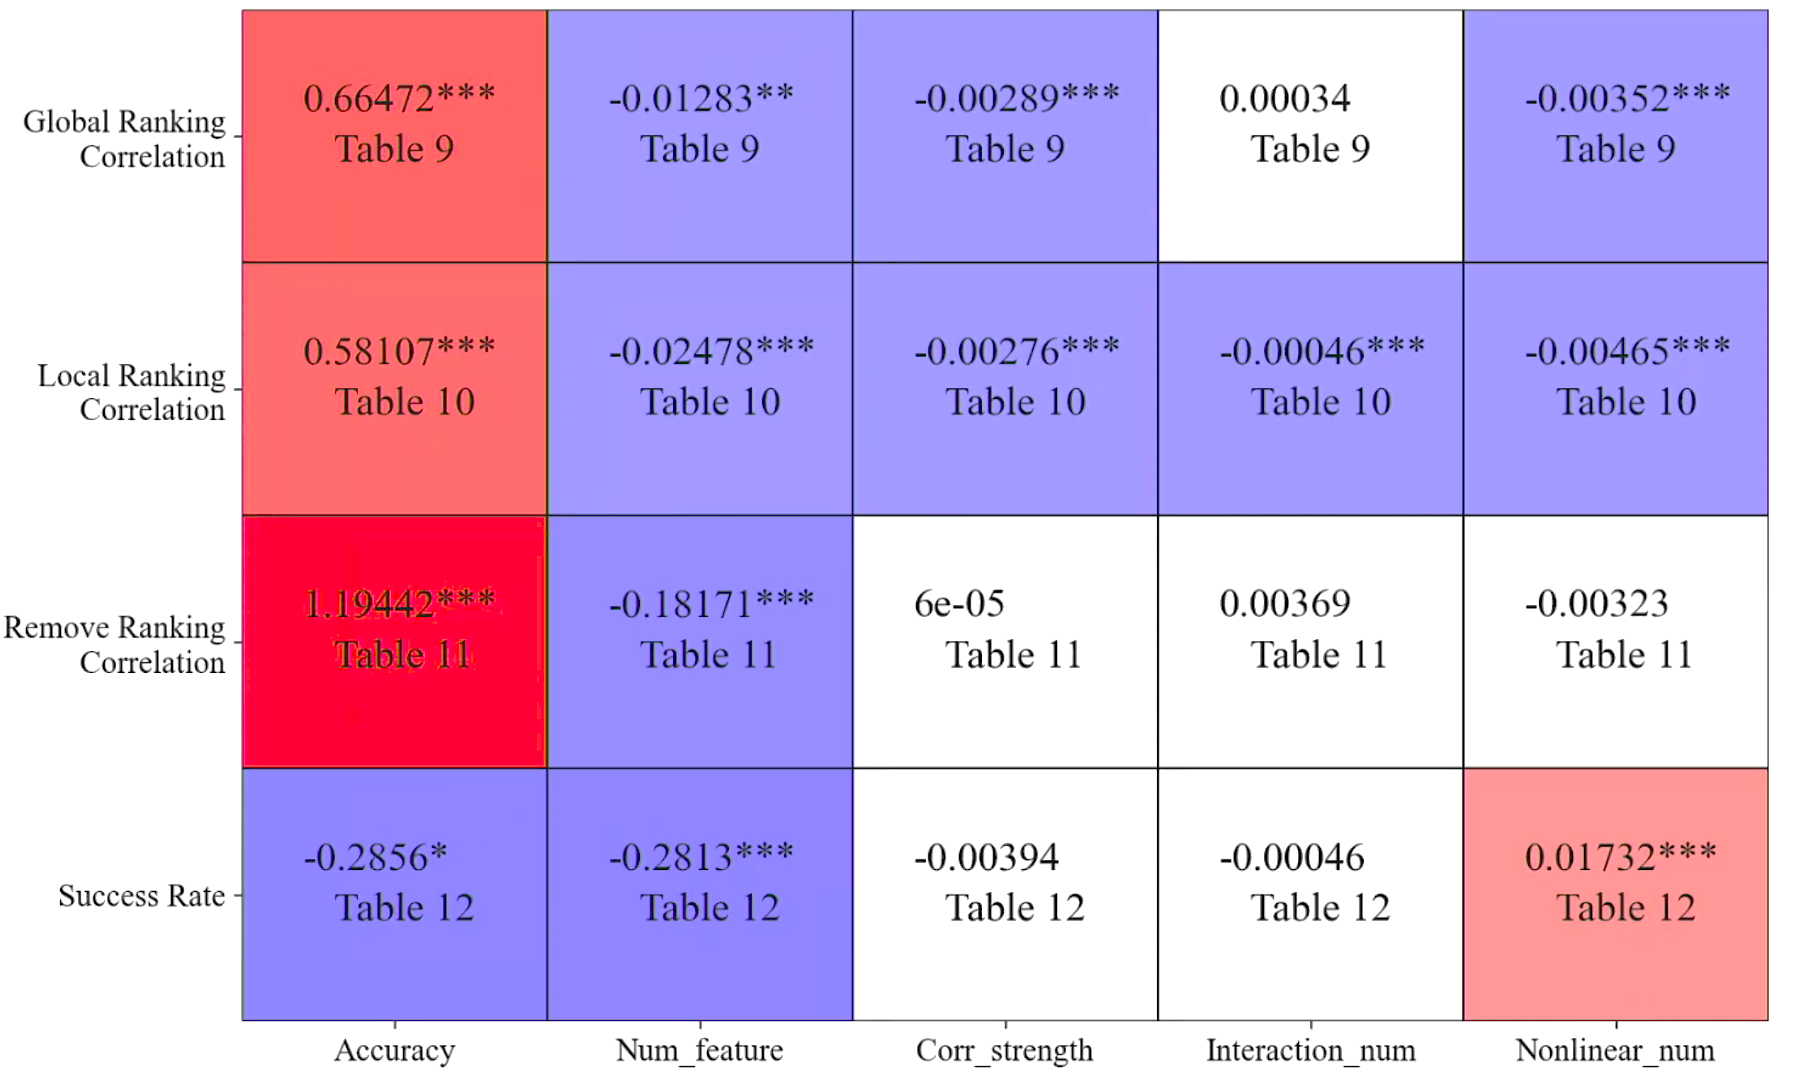
\includegraphics[width=0.7\textwidth]{Rebuttal-R1/experiment_details/media/image36_v1.png}
\caption{\textcolor{red}{Heat Map of Factor Regression Using LIME \& Spearman(Combined Regression)}}
\label{heatmap_1}
\end{figure}


\begin{figure}[h!]
\centering
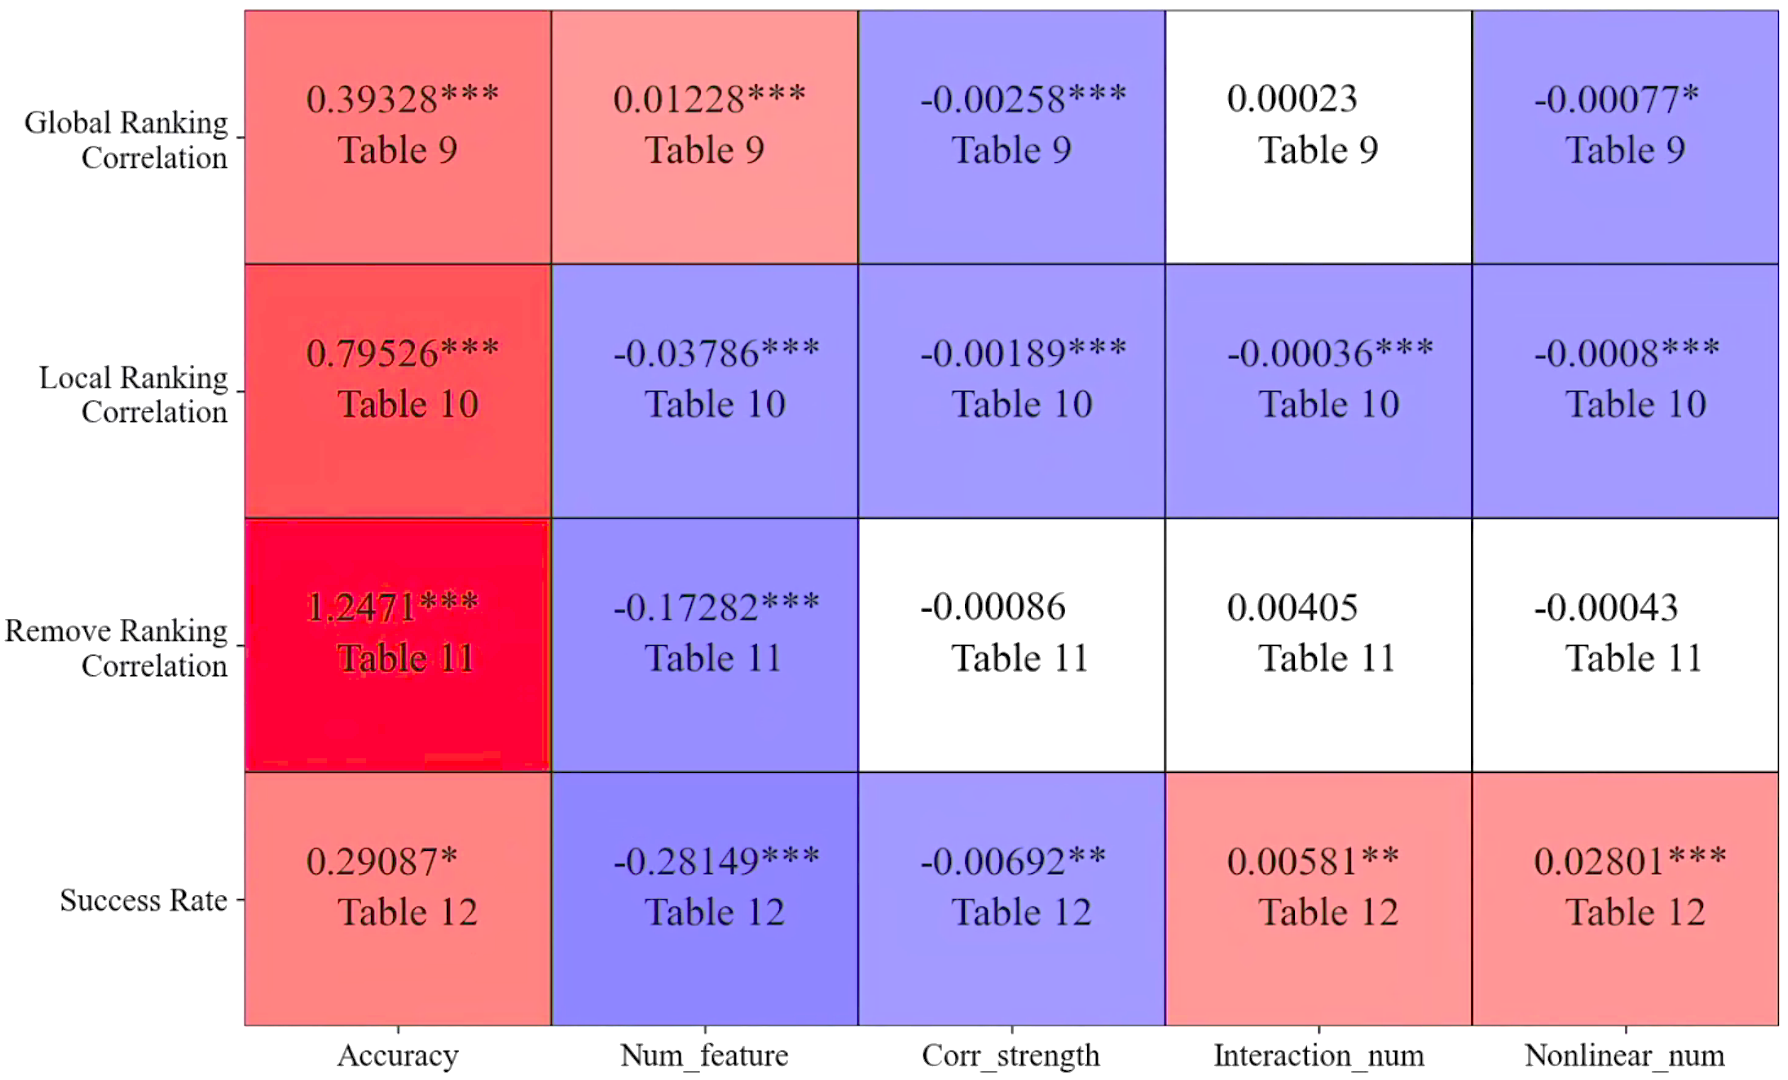
\includegraphics[width=0.7\textwidth]{Rebuttal-R1/experiment_details/media/image37_v1.png}
\caption{\textcolor{red}{Heat Map of Factor Regression Using SHAP \& Spearman(Combined Regression)}}
\label{heatmap_2}
\end{figure}

\begin{figure}[h!]
\centering
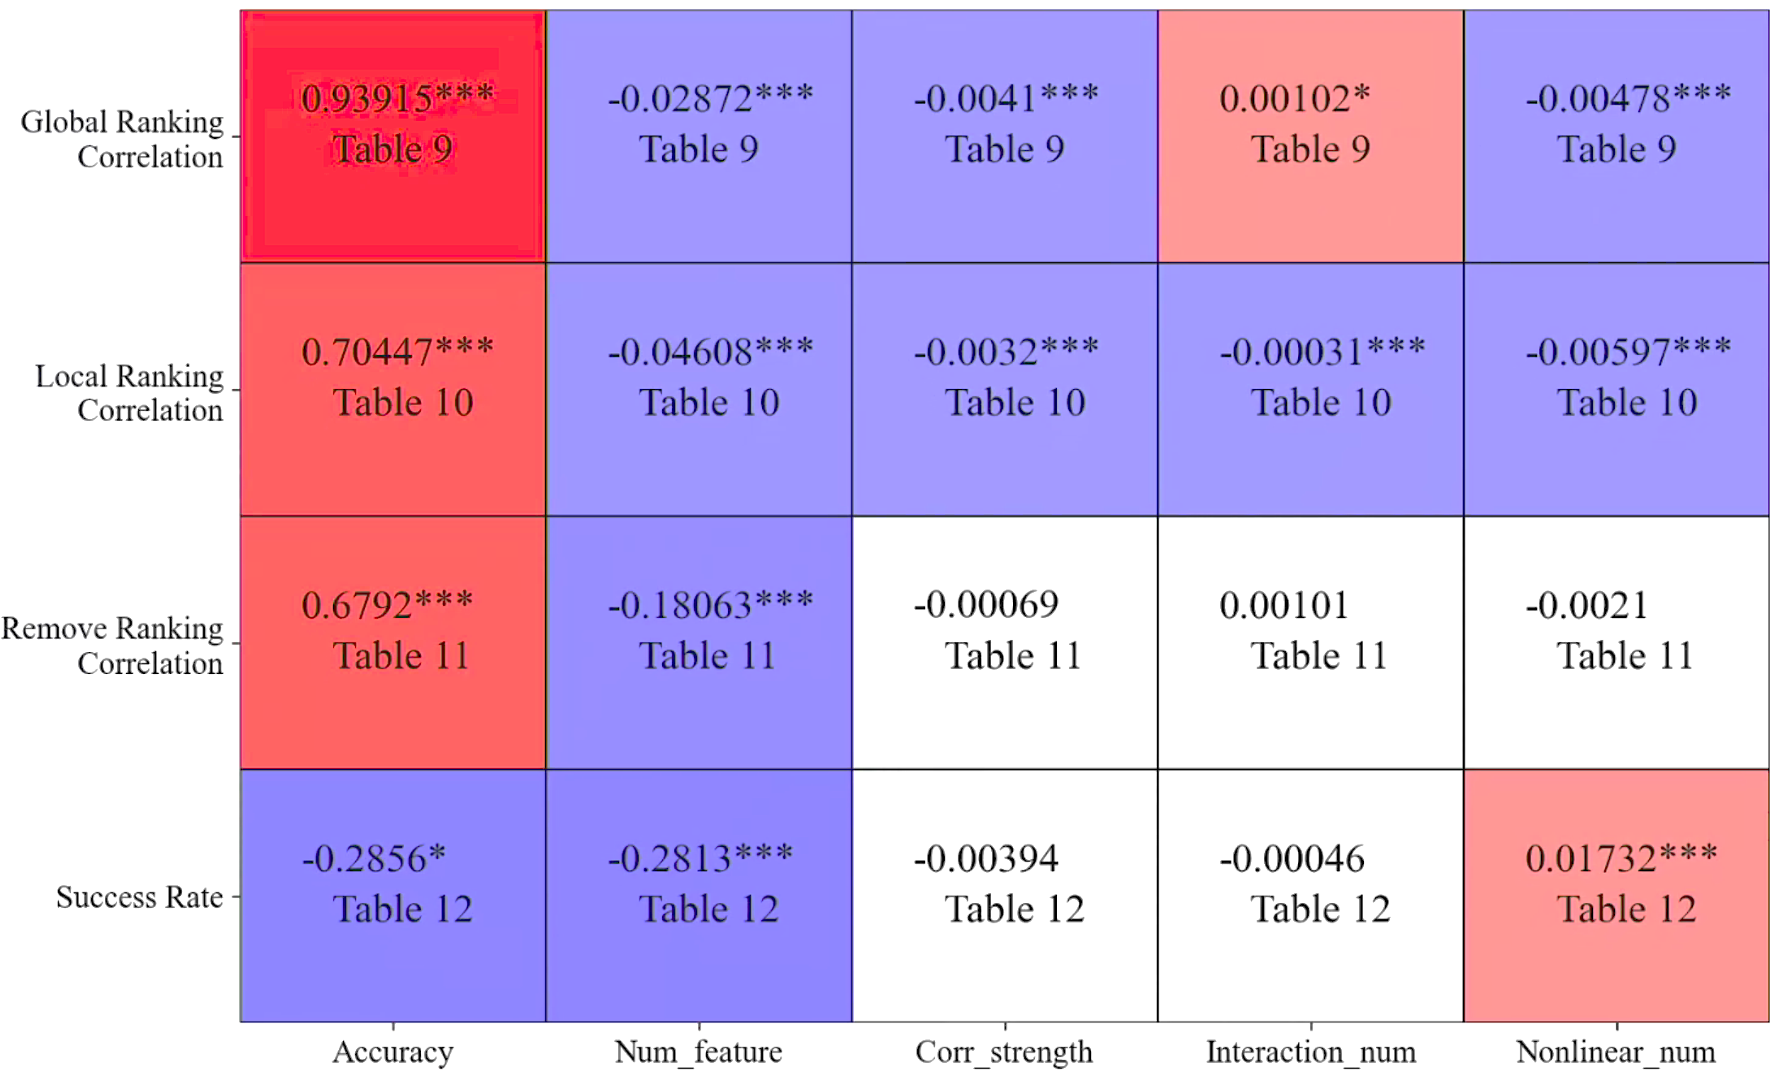
\includegraphics[width=0.7\textwidth]{Rebuttal-R1/experiment_details/media/image38_v1.png}
\caption{\textcolor{red}{Heat Map of Factor Regression Using LIME \& Spearman(Combined Regression)}}
\label{heatmap_3}
\end{figure}

\begin{figure}[h!]
\centering
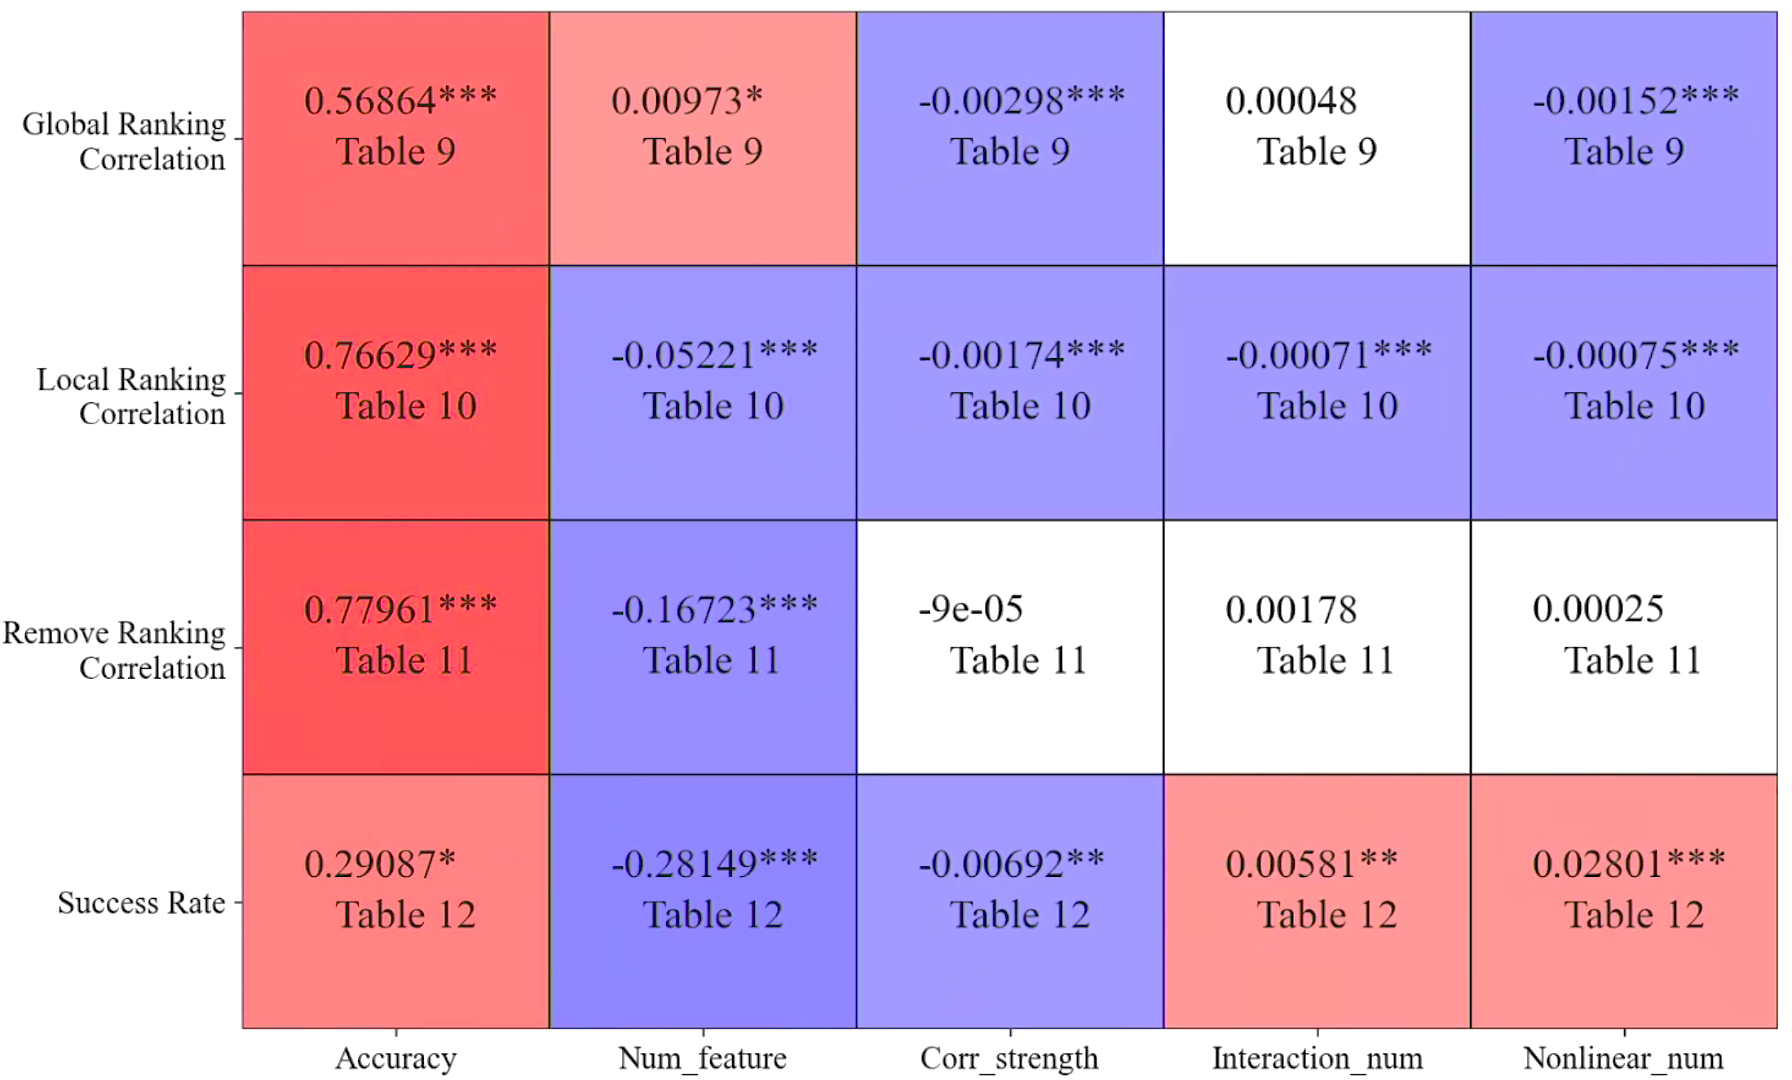
\includegraphics[width=0.7\textwidth]{Rebuttal-R1/experiment_details/media/image39_v1.png}
\caption{\textcolor{red}{Heat Map of Factor Regression Using SHAP \& Kendall Tau (Combined Regression)}}
\label{heatmap_4}
\end{figure}